\documentclass[12pt,a4paper]{article}
\usepackage[utf8]{inputenc}
\usepackage[french]{babel}
\usepackage[T1]{fontenc}
\usepackage{amsmath}
\usepackage{amsfonts}
\usepackage{amssymb}
\usepackage{graphicx}
\usepackage[left=1cm,right=1cm,top=2cm,bottom=2cm]{geometry}
\author{KONDI Abdoul malik \\ NGANDEU NDJEUKAM Alhasan}
\title{Étude prévisionnel du projet de gestion d'une librairie}
\begin{document}
\maketitle
\tableofcontents
\newpage

\section{Planning}

\begin{center}
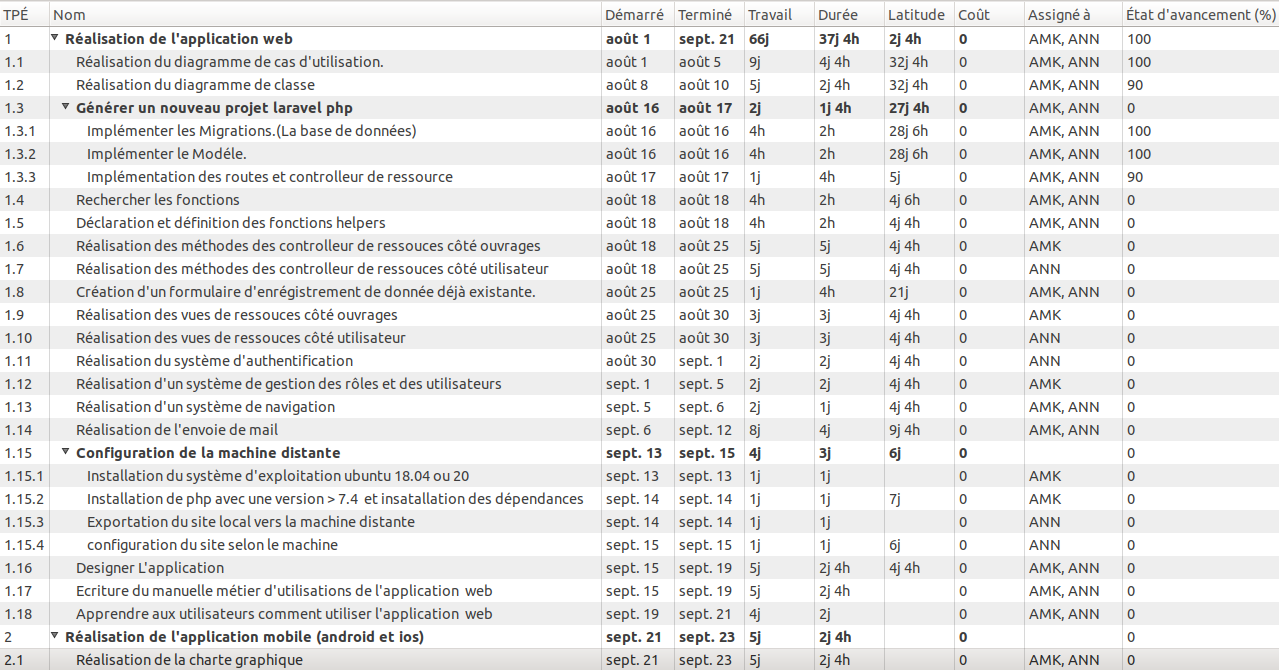
\includegraphics[scale=0.43]{images/taches.png}
\end{center}

\newpage

\section{Résumé récapitulatif du planning:}
\begin{center}
\begin{tabular}{|p{2.2cm}|p{2.2cm}|p{6.5cm}|p{6.5cm}|}
\hline 
Début & Fin & Tâche à accomplir & Besoins des stagiaires \\ 
\hline 
\textbf{01/08/2022} & \textbf{13/08/2022} & Réalisation du modèle & maître de stage\\ 
\hline 
\textbf{15/08/2022} & \textbf{17/08/2022} & Initialisation du projet et création de la base de données & maître de stage \\ 
\hline
\textbf{18/08/2022} & \textbf{25/08/2022} & \begin{itemize}
\item[•] Ajout d'un d'un nouvelle ouvrage.
\item[•] Consulter un ouvrage.
\item[•] Rechercher un ouvrage.
\item[•] Faire l'inventaire.
\item[•] Enregistrement d'un employé(personnel).
\item[•] Enregistrement d'un nouvelle abonné.
\item[•] Gestion des utilisateurs (cas se connecter)
\item[•] Prêter un ouvrage à un abonnée.
\item[•] Restituer un prêt.
\end{itemize} & Liste des livres à la Bibliothèque \\ 
\hline 
\textbf{29/08/2022} & \textbf{02/09/2022} & \begin{itemize}
\item[•] Prolonger l'emprunt d'un ouvrage.
\item[•] Renouveler l'abonnement d'un abonné.
\item[•] Alter un abonné.
\item[•] Lire un ouvrage.
\item[•] Télécharger un ouvrage.
\item[•] consulter la liste des mes emprunts.
\item[•] consulter la liste des emprunts en cours.
\item[•] sanctionner les utilisateurs.
\end{itemize} & 
\begin{itemize}
\item[•] Livres numérique
\item[•] Documents audio visuel
\item[•] Machine distante pour l'hébergement.
\item[•] Machine physique pour le personnel de la médiathèque.
\end{itemize} \\
\hline 
\textbf{05/09/2022} & \textbf{07/09/2022} & Designer l'application & - \\
\hline 
\textbf{08/09/2022} & \textbf{12/09/2022} & Écriture du manuel d'utilisation & - \\ 
\hline
\textbf{12/09/2022} & \textbf{14/09/2022} & Apprendre l'utilisation de l'application aux utilisateurs & personnels\\ 
\hline  
\textbf{14/09/2022} & \textbf{16/09/2022} & Réalisation de l'application mobile(android \& ios) & -\\ 
\hline 
\end{tabular} 
\end{center}



\end{document}




